
\setcounter{numques}{0}


%\setcounter{section}{1}
%
\exer{Applications directes}

\question{Implémenter la fonction \texttt{mult\_it(n:int, p:int) -> int} qui permet de calculer $n\times p$ par une méthode \textbf{itérative}. L'opération \texttt{*} est strictement interdite.}

\question{Implémenter la fonction \texttt{mult\_rec(n:int, p:int) -> int} qui permet de calculer $n\times p$ par une méthode \textbf{récursive}. L'opération \texttt{*} est strictement interdite.}

\question{Implémenter la fonction \texttt{puiss\_rec(x:float, n:int) -> float} qui permet de calculer $x^n$ par une méthode \textbf{récursive}. L'opération \texttt{**} est strictement interdite.}

\bigskip

\exer{Palindrome...}

On souhaite réaliser une fonction \texttt{miroir} dont le but est de retourner le <<miroir>> d'une chaîne de caractères. 
Par exemple le résultat de \texttt{miroir("miroir")} serait \textsl{''riorim''}.

\question{Programmer la fonction \texttt{miroir\_it} permettant de répondre au problème de manière itérative.}

\question{Programmer la fonction \texttt{miroir\_rec} permettant de répondre au problème de manière récursive.}

\question{Que renvoie la fonction si la chaîne de caractère est "Eh ! ça va la vache" ?}

\textit{On rappelle qu'il est possible de réaliser des opérations de slicing avec des chaînes de caractères. Ainsi si \texttt{ch='abcdef'},  et \texttt{var=ch[1:3]} alors \texttt{var} contient \texttt{'bc'}.}

\bigskip

\exer{Suite de Fibonacci}

On définit la suite de Fibonacci de la façon suivante : $
\forall n\in \mathbb{N}, \left\{ \begin{array}{l}
u_0 = 0, u_1 = 1 \\
u_{n+2} = u_{n} + u_{n+1}
\end{array}\right.
$.

\question{Définir la fonction \texttt{fibonacci\_it} permettant de calculer $u_n$ par une méthode itérative. }

\question{Définir la fonction \texttt{fibonacci\_rec} permettant de calculer $u_n$ par une méthode récursive << 
intuitive>>. }

\question{Observer comment passer du couple $(u_n,u_{n+1})$ au couple $(u_{n+1},u_{n+2})$. En déduire une autre méthode récursive pour calculer le nième terme de la suite de Fibonacci. }



\exer{Problème}

\begin{minipage}[c]{.7\linewidth}
On démontre que sur l'ensemble $\mathbb{N}\times \mathbb{N}$ est dénombrable en numérotant chaque couple $(x,y)\in\mathbb{N}^2$ suivant le procédé suggéré par la figure ci-contre.

\question{Rédiger une fonction récursive qui retourne le numéro du point de coordonnées $(x,y)$.}

\question{Rédiger la fonction réciproque, là encore de façon récursive.}
\end{minipage}\hfill
\begin{minipage}[c]{.25\linewidth}
\begin{center}
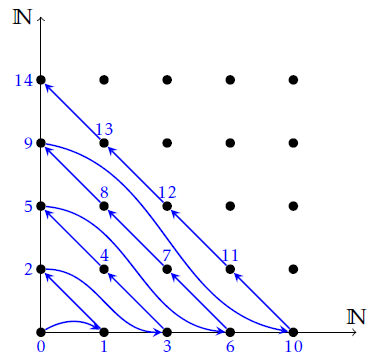
\includegraphics[width=\linewidth]{fig_01}
\end{center}

\end{minipage}

\exer{Flocon de Von Koch -- Exercice corrigé}



Dans cet exercice, vous utiliserez des tableaux \textbf{numpy} pour représenter les points. C'est plus pratique que les 
listes python pour faire les calculs vectoriels.

\begin{itemize}
\item Si $a$ et $b$ représentent respectivement les points $(x,y)$ et $(x',y')$ alors $a+b$ représente le point 
$(x+x',y+y')$.
\item Si $r$ est un réel et $a$ représente le point de coordonnées $(x,y)$ alors $r*a$ représente le point $(rx,ry)$.
\item Si $a$ et $b$ sont des tableaux \textbf{numpy} alors $dot(a,b)$ représente le produit matriciel $a\times b$ (si ce 
produit est possible). La fonction \textbf{dot} est une fonction \textbf{numpy}.
\end{itemize}

Le mathématicien suédois Von Koch a défini la courbe du même nom dont voici les premières itérations.

\begin{center}
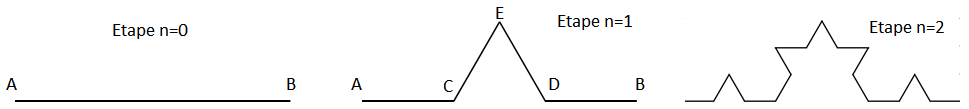
\includegraphics[width=.95\linewidth]{images/etapes_flocon}
\end{center}

\question{Ecrire une fonction \texttt{rotation} d'argument un réel \texttt{alpha} qui renvoie le tableau \textbf{numpy} 
correspondant à la matrice de rotation d'angle \texttt{alpha}.}

\question{Pour l'étape $n=1$, exprimer les points $C$ et $D$ en fonction de $A$ et $B$.}

\question{En utilisant une matrice de rotation, exprimer $E$ en fonction de $C$ et $D$.}


\question{En déduire une fonction récursive \texttt{koch} d'arguments les points \texttt{A} et \texttt{B} et un entier 
\texttt{n}. Cette fonction tracera la courbe de Von Koch pour l'itération $n$ à partir des points $A$ et $B$.}

\question{Ecrire une fonction \texttt{flocon} d'arguments les points $A$ et $B$ et un entier $n$. Cette fonction tracera 
le flocon de Von Koch pour l'itération $n$ à partir des points $A$ et $B$.}

%\begin{center}
%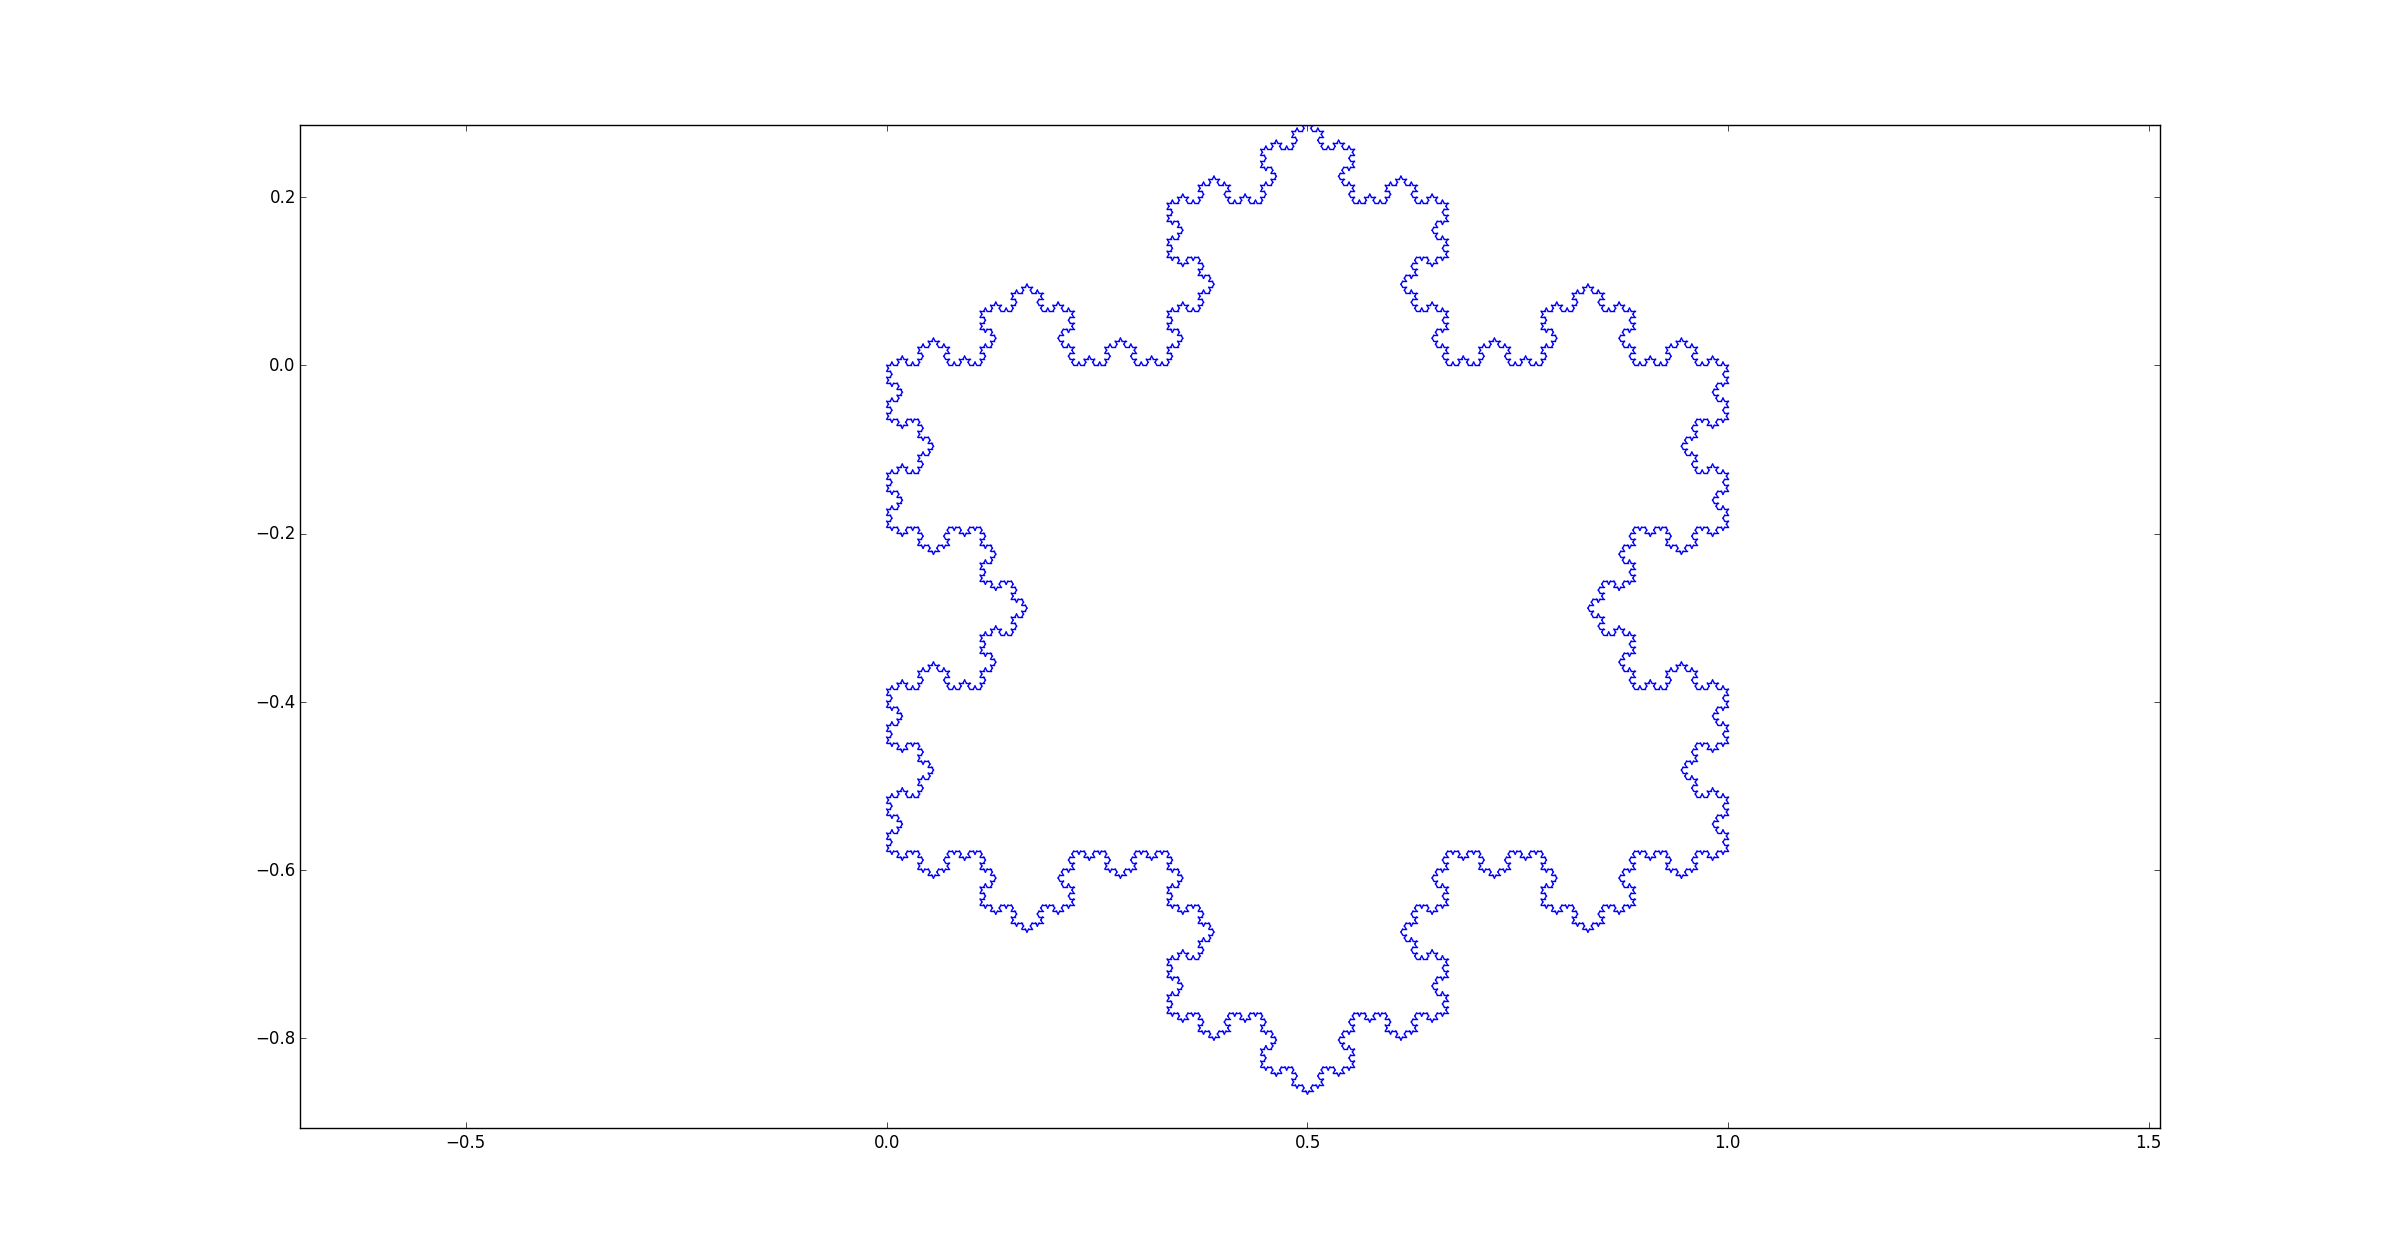
\includegraphics[width=.95\linewidth]{images/flocon_von_koch}
%\end{center}

\begin{lstlisting}
import numpy as np
import matplotlib.pyplot as plt
def rotation(angle):
    return np.array([[np.cos(angle),-np.sin(angle)],[np.sin(angle),np.cos(angle)]])
def koch(a, b, n):
    R = rotation(np.pi/3)
    if n == 0:
        plt.plot([a[0], b[0]], [a[1], b[1]],'b')
    else:
        c=np.array([(b[0]-a[0])/3+a[0],(b[1]-a[1])/3+a[1]])
        d=np.array([2*(b[0]-a[0])/3+a[0],2*(b[1]-a[1])/3+a[1]])
        vecteur=d-c
        e=np.dot(rotation(np.pi/3),vecteur)+c
        koch(a, c, n - 1)
        koch(c, e, n - 1)
        koch(e, d, n - 1)
        koch(d, b, n - 1)     
def flocon(a,b,n):
    koch(a,b,n)
    vecteur=b-a
    c=np.dot(rotation(-2*np.pi/3),vecteur)+b
    koch(b,c,n)
    koch(c,a,n)
n = 5
a = np.array([0,0])
b = np.array([1,0])
flocon(a, b, n)
plt.axis('equal')
plt.show()
\end{lstlisting}


